\section{Theorie}
\subsection{Semiklassische Herleitung}
Ein Hg-Atom welches ein Photon absorbiert kann als ein gedämpfter oszillierender Dipol beschrieben werden. Die Dipolachse ist dabei parallel zur Polarisation des absorbierten Photons. Zur Bestimmung der gesamt Intensität eines einzelnen angeregten Atoms muss über alle Zeiten integriert werden wodurch sich folgende Gleichung ergibt.
\begin{equation}
	I=C\cdot \int_{0}^{\infty}sin(\phi)^2e^{-\frac{t}{\tau}}dt
\end{equation}
Hierbei ist zu erkennen das die Strahlungscharakteristik proportional zu $sin(\phi)^2$ ist, wobei $\phi$ der Winkel zischen Dipolachse und Beobachtungsrichtung ist. Der Faktor $e^{-\frac{t}{\tau}}$ beschreibt die Dämpfung.\par
Wenn nun ein Magnetfeld angelegt wird und dieses senkrecht auf der Oszillation-Achse liegt so wird ein Drehmoment auf den Dipol ausgeübt. Dieses führt zur Präzision des Dipols und des magnetischen Moments welches hier als starr zusammenhängend betrachtet wird. Für das magnetische Moment $\mu$ eines Niveaus mit Drehimpulsquantenzahl J gilt
im schwachen Feld folgende Bewegungsgleichung:
\begin{equation}
\frac{d\vec{\mu}}{dt}=\frac{\omega_L}{B}\vec{\mu}\times\vec{B}
\label{Präzesion}
\end{equation}
hierbei ist $\omega_L$ die Larmorfrequenz mit:
\begin{equation}
	\omega_L=g_J\frac{\mu_B}{\hbar}B
\end{equation}
Grafisch wird die Bewegung in Abbildung \ref{Präzesionsbild} dargestellt.
\begin{figure}[ht]
	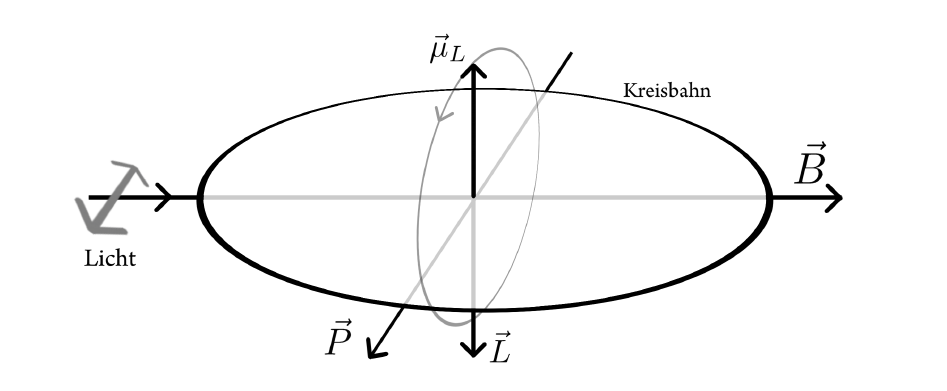
\includegraphics[scale=0.8]{Bild/TestP}
	\centering
	\caption[Semiklassische Darstellung des Hanle Effekts]{Darstellung der Präzessionsbewegung eines Elektrons mit Dipolmoment $\vec{P}$, Drehimpuls $\vec{L}$ und magnetischem Moment $\mu_L$ bei angelegtem Magnetfeld der Flussdichte $B$.\cite{anleitung}}
	\label{Präzesionsbild}
\end{figure}\\
Sind Polarisation (und somit auch Dipolachse) zum Zeitpunkt der Absorption parallel zur Beobachtungsebene gilt $\theta(t)=\omega_Lt$ mit $\theta(t=0)=0$. Das bedeutet für die Intensität:
\begin{equation}
	I=C\cdot \int_{0}^{\infty}\sin(\omega_Lt)^2e^{-\frac{t}{\tau}}dt=\frac{C\tau}{2}\left(\frac{(2\omega_L\tau)^2}{1+(2\omega_L\tau)^2}\right)
	\label{GLStuff}
\end{equation}
Ist die Beobachtungsrichtung zum Zeitpunkt der Absorption senkrecht zur Polarisationsrichtung gilt: $\theta(t)=\omega_Lt+\frac{\pi}{2}$ mit $\theta(t=0)=\frac{\pi}{2}$. Die Intensität lässt sich ähnlich wie in Gleichung \ref{GLStuff} beschreiben:
\begin{equation}
I=C\cdot \int_{0}^{\infty}\cos(\omega_Lt)^2e^{-\frac{t}{\tau}}dt=\frac{C\tau}{2}\left(2-\frac{(2\omega_L\tau)^2}{1+(2\omega_L\tau)^2}\right)
\label{GLStuff2}
\end{equation}
Die Gleichung \ref{GLStuff} entspricht einer inversen Lorenz-kurve und Gleichung \ref{GLStuff2} einer normalen. Die Lebensdauer $\tau$ dieser Kurven kann über die Breite der Funktion auf halber Höhe (\textit{eng: Full width at half maximum (FWHM)}) bestimmt werden (siehe Abb.\ref{Lorenzbild}). Hierfür gilt:
\begin{equation}
	\tau=\frac{\hbar}{g_J\mu_BB_{FW}}
	\label{tau}
\end{equation}
\begin{figure}[ht]
	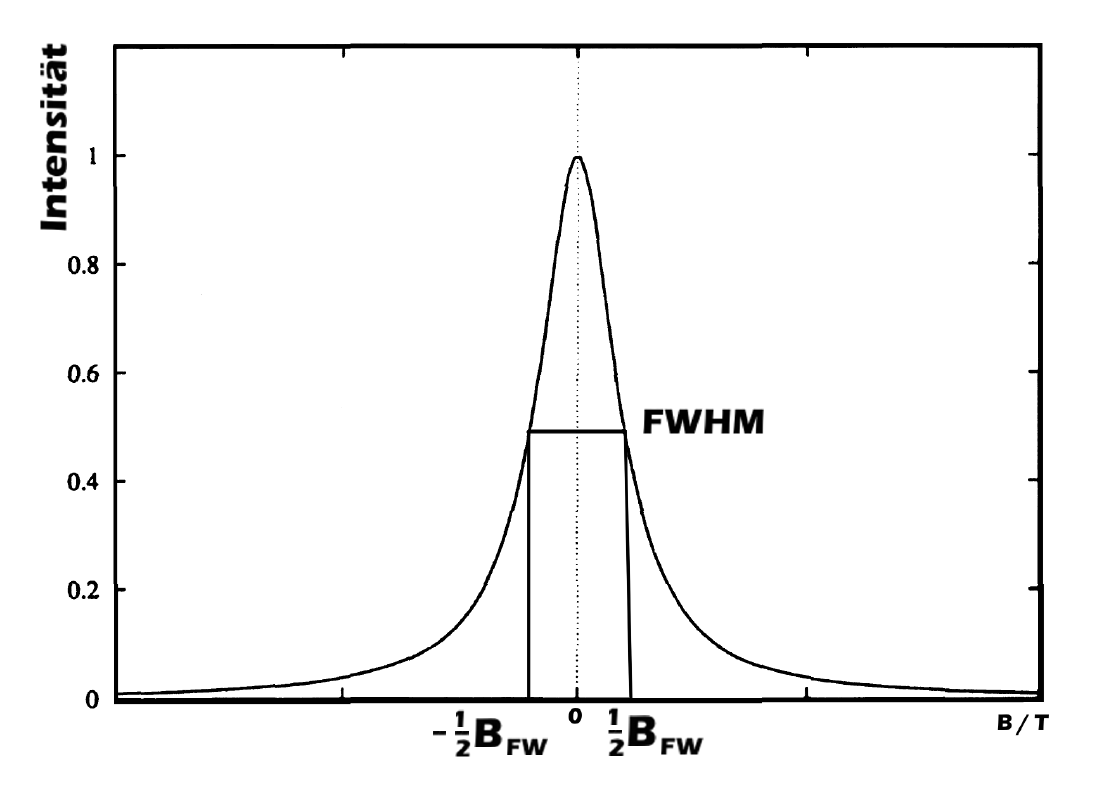
\includegraphics[scale=0.7]{Bild/Lorenz}
	\centering
	\caption[Lorentzkurve]{Lorentzkurve mit sichtbare Intensität in Beobachtungsrichtung $0^\circ$ mit FWHM eingezeichnet.\cite{anleitung}}
	\label{Lorenzbild}
\end{figure}
Durch das einfügen einer Phase in Gleichung \ref{GLStuff2} kann man die Gleichung \ref{EasyFit} erhalten die von dem Winkel unabhängig ist. Durch einen Fit kann man hier direkt $\tau$ ablesen.
\begin{equation}
I=C\cdot \int_{0}^{\infty}\cos(\omega_Lt+\phi)^2e^{-\frac{t}{\tau}}dt=\frac{C\tau}{2}\left(\frac{1+(2\tau\omega_L)^2+\cos(2\phi)-2\omega_L\tau\sin(2\phi)}{1+(2\tau\omega_L)^2}\right)
\label{EasyFit}
\end{equation}
\subsection{Quantenmechanische Erklärung}
In der Quantenmechanik wird das Phänomen der Resonanzfluoreszenz durch Interferenz sich überlagernder Zustände beschrieben. Zustände unterschiedlicher magnetischer Quantenzahl $m_j$ sind im Allgemeinen erst einmal energetisch gleich, “entartet“. Die Entartung kann aber durch Anlegen eines Magnetfeldes aufgehoben werden (Zeeman-Effekt). In Spezialfällen verursacht die Kreuzung zweier Niveaus von Zuständen verschiedener Gesamtdrehimpulse, bei bestimmten Magnetfeldstärken, eine weitere Entartung. 
\begin{figure}[ht]
	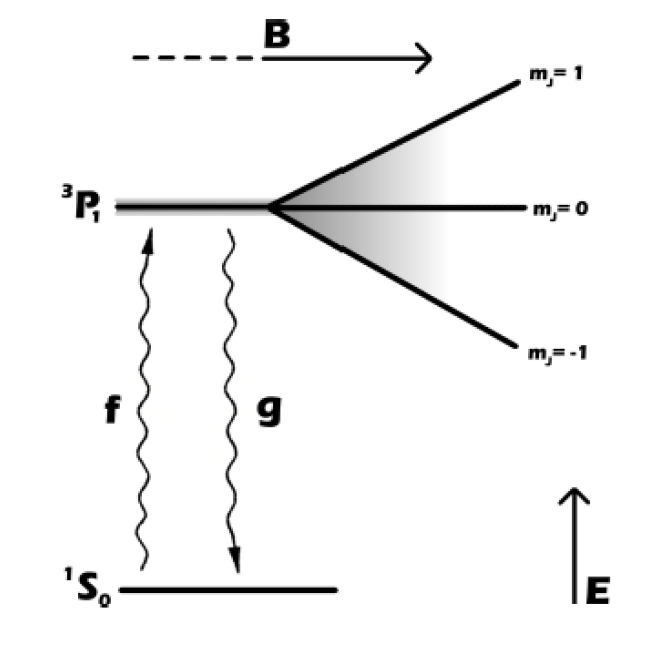
\includegraphics[scale=0.6]{Bild/Zeeman}
	\centering
	\caption[Zeeman-Effekt]{Aufspaltung der Energieniveaus durch $m_j$ in einem Magnetfeld.\cite{anleitung}}
\end{figure}
Liegt keine Energieaufspaltung vor werden die Niveaus kohärent angeregt werden und bei Abregung kommt es zur Interferenz mehrerer Zustände des selben Atoms. Damit gilt:
\begin{equation}
	I\propto(A_1+A_2)^2
\end{equation}
Bei einer Aufspaltung der Niveaus können die Niveaus getrennt angeregt und abgeregt werden. Für die gesamt Intensität gilt dann:
\begin{equation}
I\propto A_1^2+A_2^2
\end{equation}
\subsubsection{Breit-Formel}
Zur quantenmechanischen Auswertung wird eine allgemeine Formel zur Resonanzfluoreszenz von G.Breit und P.Franken. Die Formel beschreibt die Rate mit der Photonen einer linearen Polarisationsrichtung $\vec{g}$ emittiert wenn die Probe mit in $\vec{f}$ polarisiertes Licht gestrahlt wird. Die Gleichung, hier ohne Herleitung lautet:
\begin{equation}
	R(\vec{f},\vec{g})=N\int_{0}^{\infty}R(\vec{f},\vec{g},t)dt=N\sum_{m,m'}^{\mu,\mu'}\frac{f_{m\mu}f_{\mu'm}g_{\mu m'}g_{m',\mu'}}{L_{\mu,\mu'}-i(\omega_\mu -\omega_\mu')}
\end{equation}
Eine genauere Herleitung findet sich in der Versuchsanleitung\cite{anleitung} oder in der 'Interfernce Effects in the Resonance Fluorescence of "Crossed" Exited Atomic States' by P.A.Franken.\cite{Franken} \par
Diese Formel für das hier durchgeführte Experiment auf den Übergang von $^3P_1$ auf den $^1S_0$ Zustand angewendet. Daraus ergibt sich wie in der Versuchsanleitung \cite{anleitung} beschrieben die Form:
\begin{equation}
R=C\frac{1}{1+(2\omega_L\tau)^2}
\end{equation}
Diese entspricht dem Semiklassischen Ergebnis in Gleichung \ref{GLStuff}.
\subsection{Coherence Narrowing und Dampfdruck}
Coherence Narrowing bezieht sich auf den Effekt, dass ein von einem Atom emittiertes Photon ein weiteres Atom anregt. Dieses Atom würde nun die gleiche Präzessionsbewegung machen und wieder ein identisches Photon aussenden. Dies führt dazu, dass bei genügend großen Streuquerschnitt sich dieser Prozess mehrfach wiederholen kann. Durch die Ununterscheidbarkeit der Photonen wird die Lebenszeit künstlich erhöht. Um diesen Effekt zu eliminieren werden die Messungen bei variierendem Druck durchgeführt und die tatsächliche Lebensdauer aus der Extrapolation für den Druck $p = 0$ bestimmt. Da der Druck im System nicht messbar ist, muss er mit folgender empirisch bestimmten Formel aus
der Temperatur berechnet werden: 
\begin{equation}
	\ln(\frac{p}{p_c})=(\frac{T_c}{T})(a_1T_r+a_2T_r^{1.89}+a_3T_r^2+a_4T_r^8+a_5T_r^{8.5}+a_6T_r^9)
	\label{Coherence}
\end{equation}
Die Konstanten für kritischen Druck und kritische Temperatur sind:
 $$p_c=167000\,\text{Pa}$$
 $$T_c=1764\,\text{K}$$
Die Parameter $a_i$ sind:
$$a_1=-4,57618368, \qquad a_2 = -1.40726277, \qquad a_3 = 2.36263541$$
$$a_4 = -31,0889985, \qquad a_5 = 58,0183959,\qquad a_6 = -27,6304546$$
\subsection{Versuchsaufbau}
Der Versuchsaufbau sieht wie in Abbildung:\ref{VAufbau} gezeigt aus. Zu Beginn wird Licht aus einer Quecksilberdampflampe genommen und durch eine Linse fokussiert mit der Hilfe eines Interferenzfilters wird dann die gesuchte Wellenlänge von herausgefiltert. Daraufhin wird ein Polarisationsfilter genutzt um die Polarisation des Lichtes einzustellen. Hiernach wird das Licht auf die Quecksilber Probe fokussiert mit einer weiteren Linse. Senkrecht zum Strahlengang befindet sich der Photomultiplier welcher als Detektor der emittierten Photonen genutzt wird. Die Quecksilber probe wird über Wärmeleitungen (HP) mit Peltierelementen verbunden welche die Probe kühlen. Um das Magnetfeld zu kontrollieren wird eine Anordnung von Helmholtz-Spulen verwendet. Hierbei werden einmal die Felder in $y,z$ Richtung eliminiert. Die Spule die das Feld in $x$ Richtung verändert wird zum Durchfahren des Feldes genutzt um die Zeeman Aufspaltung zu erreichen welche letztendlich das Hanle-Signal generiert. Hierzu wird ein Rampengenerator verwendet der die Spannung die an der Helmholtz-Spule anliegt langsam verändert wodurch sich die Lorentzkurve bei Richtiger Polarisationseinstellung ausbildet.
\begin{figure}[ht]
	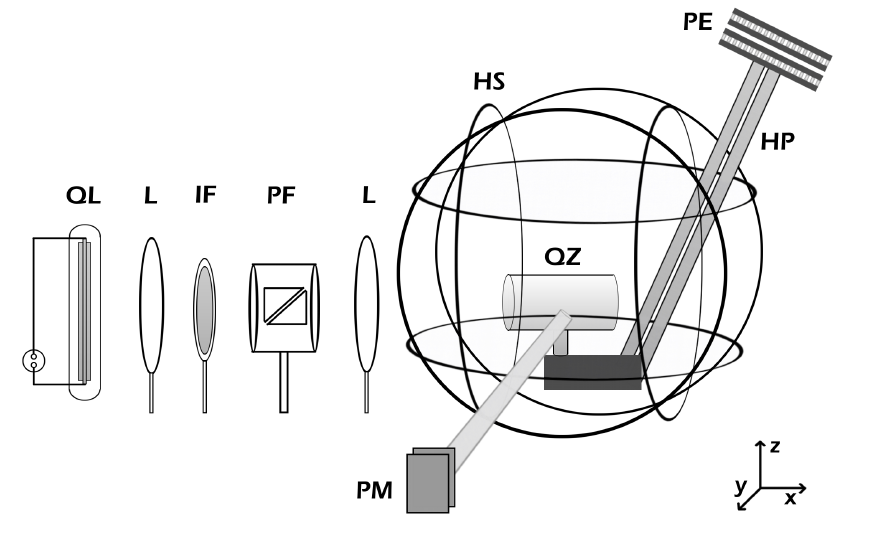
\includegraphics[scale=0.9]{Bild/VAufbau}
	\centering
	\caption[Versuchsaufbau]{Versuchsaufbau des Experiments. Quecksilberdampflampe (QL), Linse (L), Interferenzfilter (IF), Polarisationsfilter (PF), Quecksilberdampf-Resonanzzelle (QZ), Heatpipes (HP), Peltierelemente (PE), Helmholtz-spulen (HS), Photomultiplier (PM). \cite{anleitung}}
	\label{VAufbau}
\end{figure} 
\FloatBarrier
\section{Versuchsdurchführung}
Zu beginn des Experiments musste als erstes die Magnetfelder in $y$ und $z$ Richtung so kalibriert werden, dass diese das Erdmagnetfeld kompensieren. Dafür musste am Polarisationsfilter die $0^\circ$ Einstellung gefunden werden. Durch das Durchfahren des Feldes in x Richtung erkennt man bei $0^\circ$ eine Lorentzkurve. Diese muss durch Veränderung des Stroms der Helmholtz Spulen in $y$ und $z$ verbessert werden. So war zu Beginn die Kurve nicht sehr symmetrisch. Dies wurde nochmal für $90^\circ$ durchgeführt, was sich an vielen Stellen als sehr schwierig und Zeitaufwendig herausstellte. Besonders bei $45^\circ$ wurde keine besonders schöne Symmetrie erreicht.
\begin{align}
	I_y=(-0.0217\pm0.0001)\,\text{A}
	\label{comp_curr}
\end{align}
\begin{align}
	I_z=(-0.2957\pm0.0001)\,\text{A}
	\label{comp_curr2}
\end{align}
Nachdem eine geeignete Einstellungen (vgl.\ref{comp_curr},\ref{comp_curr2}) gefunden wurden, wurden bei $0^\circ$ $15$ Messungen der Lorentzkurve gemacht. Danach wurde das System mit Hilfe der Peltierelemente stückweise abgekühlt, um die Kurven für die Unterschiedlichen Polarisationsrichtungen bei verschiedenen Temperaturen, beziehungsweise Drücken, gemessen. Aus Zeitgründen wurde diese erste Messung kurzgehalten und anschließend eine Messung bei steigender Temperatur durchgeführt. Am nächsten Tag wurde nochmal eine Kühlmessung mit mehr Messpunkten aufgenommen.
